\let\negmedspace\undefined
\let\negthickspace\undefined
\documentclass[journal]{IEEEtran}
\usepackage[a5paper, margin=10mm, onecolumn]{geometry}
%\usepackage{lmodern} % Ensure lmodern is loaded for pdflatex
\usepackage{tfrupee} % Include tfrupee package

\setlength{\headheight}{1cm} % Set the height of the header box
\setlength{\headsep}{0mm}     % Set the distance between the header box and the top of the text

\usepackage{gvv-book}
\usepackage{gvv}
\usepackage{cite}
\usepackage{amsmath,amssymb,amsfonts,amsthm}
\usepackage{algorithmic}
\usepackage{graphicx}
\usepackage{textcomp}
\usepackage{xcolor}
\usepackage{txfonts}
\usepackage{listings}
\usepackage{enumitem}
\usepackage{mathtools}
\usepackage{gensymb}
\usepackage{comment}
\usepackage[breaklinks=true]{hyperref}
\usepackage{tkz-euclide} 
\usepackage{listings}
% \usepackage{gvv}                                        
\def\inputGnumericTable{}                                 
\usepackage[latin1]{inputenc}                                
\usepackage{color}                                            
\usepackage{array}                                            
\usepackage{longtable}                                       
\usepackage{calc}                                             
\usepackage{multirow}                                         
\usepackage{hhline}                                           
\usepackage{ifthen}                                           
\usepackage{lscape}
\begin{document}

\bibliographystyle{IEEEtran}
\vspace{3cm}

\title{9.6.1}
\author{EE24BTECH11001 - Aditya Tripathy}
 \maketitle
% \newpage
% \bigskip
{\let\newpage\relax\maketitle}

\renewcommand{\thefigure}{\theenumi}
\renewcommand{\thetable}{\theenumi}
\setlength{\intextsep}{10pt} % Space between text and floats


\numberwithin{equation}{enumi}
\numberwithin{figure}{enumi}
\renewcommand{\thetable}{\theenumi}


\textbf{Question}:\\
Plot a solution to the following differential equation:\\
    $y^\prime + 2y = \sin x$
\\
\textbf{Solution: }\\
To plot a curve in the solution family, we take the initial condition to be\\
$x_0 = 0, y_0 = 1$\\
Using Euler's Method, we represent the the differential equation in the following difference equations:
\begin{align}
    x_{n+1} = x_n + h\\
    y_{n+1} - y_n + 2hy_n  = h\sin x_n\\
    \xrightarrow{} y_{n+1} = \brak{1-2h}y_n + h\sin x_n
\end{align}
Now we can iteratively generate points which lie close to the graph.\\
To check how close the approximate graph is to the actual solution, we will solve the original 
equation using a Laplace Transform method:\\
Let $\mathcal{L}\brak{y} = Y$\\
\begin{align}
    \brak{sY - y_0} +2Y &= \mathcal{L}\brak{\sin x}\\
    \mathcal{L}\brak{\sin x} &= \int_{0}^{\infty} e^{-sx}\sin x = \frac{1}{s^2 + 1}\\
    \brak{s + 2}Y &= y_0 + \frac{1}{s^2 + 1}\\
    Y &= \frac{y_0}{s + 2} + \frac{1}{\brak{s^2+1}\brak{s+2}}\\
\end{align}
    Using method of partial fractions,
    \begin{align}   
        \frac{1}{\brak{s^2+1}{s+2}} = \frac{a}{s+2} + \frac{bs + c}{s^2+1}\\
    \end{align}
    On solving we get,
    \begin{align}
        a &= \frac{1}{5}\\
        b &= \frac{-1}{5}\\
        c &= \frac{2}{5}\\
    \end{align}
    \text{Substituting $y_0 = 1$},\\
\begin{align}
    Y &= \frac{1}{s + 2} + \frac{0.2}{s+2} + \frac{-0.2s}{s^2 + 1} + \frac{0.4}{s^2 + 1}\\
    \xrightarrow{} Y &=  \frac{1.2}{s + 2} + \frac{-0.2s}{s^2 + 1} + \frac{0.4}{s^2 + 1}\\
\end{align}
    \text{Now, we take the inverse laplace transform to get a solution,}\\
\begin{align}
    \mathcal{L}^{-1}\brak{\frac{1}{s+2}} &= e^{-2x}u\brak{x}\\
    \mathcal{L}^{-1}\brak{\frac{1}{s^2+1}} &= \sin xu\brak{x}\\
    \mathcal{L}^{-1}\brak{\frac{s}{s^2+1}} &= \cos xu\brak{x}
\end{align}
Therefore the final solution to the differential equation is,
\begin{align}
    y\brak{x} = \brak{1.2e^{-2x} - 0.2\cos x + 0.4\sin x}u\brak{x} 
\end{align}
For the following approximate graph, I chose $h = 0.01$ and $h = 0.1$.
\begin{figure}[h!]
   \centering
   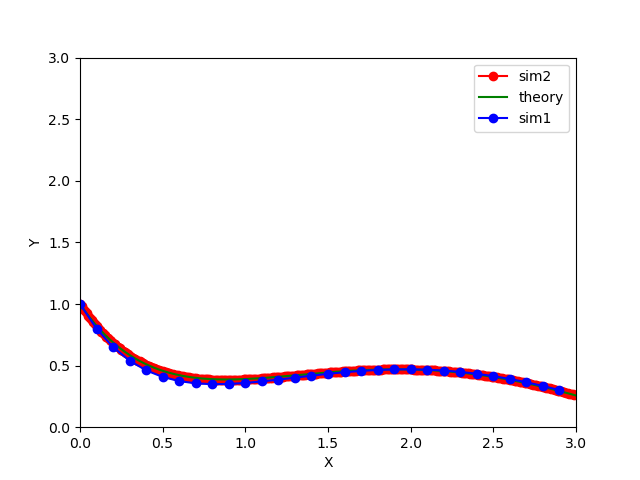
\includegraphics[width=0.7\columnwidth]{figs/fig.png}
    \caption{Approximate solution of the DE}
\end{figure}
\end{document}  
